%!TEX root = ../doc.tex
\chapter{ROS Grundlagen}
\label{sec:TheoretischeGrundlagen}
\section{Überblick}
Das Robot Operating System oder kurz ROS ist eine flexibles Framework zur Entwicklung von Software für Roboter. Es bietet eine Reihe von Funktionen, Werkzeugen und Bibliotheken. Mit diesen ist es möglich alle gängigen Operationen, welche man von einer Software von diesem Typ erwarten kann zu erledigen. Dazu gehören unter anderem Hardwareabstraktion, das Versenden von Nachrichten zwischen Prozessen und Paketmanagement.\cite{ROSIntro6:online}\\
Der Kern von ROS ist unter der 3-Klausel-BSD-Lizenz lizenziert und somit komplett Open-Source. \cite{ROSorgIs25:online} ROS darf somit von jeder Person, oder Firma verwendet und auch weiterentwickelt werden, solange die drei Klauseln\footnote{Siehe: \url{https://opensource.org/licenses/BSD-3-Clause}} der BSD-Lizenz eingehalten werden. ROS basiert genau aus diesem Grund auch aus diversen Teilprojekten, welche es seit der Entstehung von Anfang der 2000er Jahre vorangetrieben haben.\cite{Joseph2015}

\subsection{Ziele von ROS}
ROS setzt sich nicht zum Ziel ein Roboterframework zu sein, welches eine unzählige Vielfalt von Funktionen bereitstellt. Das Hauptziel von ROS ist es, dass Software welche für Roboter in der Forschung und der Entwicklung geschrieben wurde frei zugänglich ist und somit wiederverwendet werden kann. Aus diesem Grund ist ROS so aufgebaut, dass die einzelnen Komponenten respektive Funktionen lose aneinander gekoppelt werden können.
Weitere Ziele von ROS sind es, dass die für ROS entwickelte Software nicht proprietär ist, sondern auch in anderen Roboterframeworks gebraucht werden kann. Gleichzeitig soll ROS unabhängig von der Programmiersprache sein, aus diesem Grund ist es möglich ROS in \verb|C++, Python| und \verb|Lisp| zu programmieren, zudem stehen experimentelle Bibliotheken zur Verfügung mit welchen \verb|JAVA| und \verb|Lua| eingebunden werden können.\cite{Joseph2015}

\subsection{Betriebssysteme}
Momentan ist ROS nur auf Unix basierten Betriebssystemen verfügbar. Die Software von ROS wird Hauptsächlich auf Ubuntu und Mac OS X getestet, es werden aber durch die Community Support für andere Linux Distributionen wie zum Beispiel Fedora, Gentoo und Arch Linux angeboten. Eine Portierung von ROS auf Microsoft Windows ist zwar möglich, wird aber im Moment noch nicht angeboten.\cite{ROSIntro6:online}

\subsection{Distributionen}\label{sec:Distro}
Der Kern von ROS wird, ähnlich wie bei Linux Systemen, über Distributionen versioniert und verteilt. Diese Distributionen beinhalten alle für ROS gebrauchten Basispakete und Bibliotheken. Ziel dieser Distributionen ist es für Anwender eine stabile Basis zu schaffen, auf welcher aufgebaut werden kann. ROS versucht innerhalb einer Distribution keine grossen Änderungen zu vollziehen, damit plötzliche Inkompatibilitäten vermieden werden können.
\begin{table}[H]
	\centering
	\begin{tabular}{lll}
		\textbf{Distro}      & \textbf{Erscheinungsdatum} & \textbf{EOL Datum}     \\ \hline
		ROS Lunar Loggerhead & 23 May 2017                & Mai 2019               \\
		ROS Kinetic Kame     & 23 May 2016                & April 2021(Xenial EOL) \\
		ROS Jade Turtle      & 23 May 2015                & Mai 2017               \\
		ROS Indigo Igloo     & 22 Juli 2014               & April 2019(Trusty EOL)
	\end{tabular}
	\caption[Übersicht der noch gewarteten ROS Distributionen]{Übersicht der noch gewarteten ROS Distributionen\cite{Saito2017}}
	\label{tab:ROSDistros}
\end{table}
 
\section{ROS Dateisystemebene} \label{sec:ROSDateisystemeben}
Die Dateisystemebene repräsentiert die Daten, welche auf der Festplatte abgespeichert sind. Die Dateisystemebene beinhaltet auch Konzepte, um den Aufbau von Packages einheitlich zu gestalten.
\subsection{Packages} \label{sec:Packages}
Packages sind der einfachste Organisationsbaustein in ROS, Ziel von Packages ist es für ROS-Anwender eine Struktur zu schaffen, welche einfach einsehbar und gut wiederverwendbar ist. Ein Package kann Nodes, unabhängige Bibliotheken, Datasets, Konfigurationsfiles, nicht ROS-Spezifischer Code und vieles anderes enthalten. In einem Package sind Typischerweise folgende Unterordner und Files zu finden.

\begin{description}[align=left]
	\item[include/package\_name] Headers von \verb|C++| Files
	\item[launch/] Ordner welcher .launch-Files enthält welche ein oder mehrere Nodes starten können
	\item[msg/] Ordner der .msg-Files enthält
	\item[srv/] Ordner der .srv-Files enthält
	\item[scripts/] Ordner der ausführbare Skripts enthält
	\item[CMakeLists.txt] CMake Build File (siehe \ref{sec:catkinCMakeLists})
	\item[Package.xml] catkin Package File (siehe \ref{sec:catkinPackageFile})
	\item[Changelog.rst] Einige Pakete enthalten ein Änderungsprotokoll
\end{description}

\subsection{Metapackages}
Ein Metapackage ist eine Untergruppe eines Normalen Packages. Sie dienen nur dazu, eine Gruppe von verwandten Paketen darzustellen. 

\subsection{Repositories}
Die meisten ROS-Packages werden durch ein \gls{VCS} verwaltet. Eine Gruppe von Packages, welche mit dem selben VCS verwaltet wird, wird in einem Repository zusammengefasst. Es ist auch möglich, dass ein Repository nur ein einzelnes Paket beinhaltet.


\section{ROS Berechnungsebene}
Die Berechnungsebene in ROS ist aufgebaut auf einem Peer-to-Peer Netzwerk aus einzelnen Prozessen, die Zusammenarbeit dieser einzelnen Prozessknoten ermöglicht es, dass komplexe Probleme gelöst werden können. Die Basis des auf dem TCP/IP-Protokoll aufgebauten Netzwerkes bilden Nodes, ROS-Master, Parameterserver, Messages, Topics, Services, Actions und Bags. All diese Komponenten tragen auf eine Art der Datenverarbeitung bei.

\subsection{Nodes}
Ein ausführbarer Prozess wird in ROS als Node bezeichnet. Ein Node kann Tasks und Berechnungen ausführen, sowie über das ROS-Netzwerk kommunizieren. Jeder Node arbeitet  individuell und ist mit einem TCP-IP-Socket verbunden. Dies erlaubt es, dass ein Absturz eines Nodes nicht einen Systemabsturz herbeiführt. Deshalb ist es auch zu empfehlen die Nodes so zu gestalten, dass jeder Node einen spezifischen Task erledigt und nicht ein Node mehrere Aufgaben hat, zudem wird durch die Aufteilung der Aufgaben die Komplexität des Codes tief gehalten.\cite{Conley2013}

\subsection{ROS-Master}
Der ROS-Master stellt für alle Nodes im ROS-System Registrierungs- und Namensservices zur Verfügung. Die Aufgabe des ROS-Masters ist es dabei Publisher und Subscriber zu bestimmten Topics, sowie Services zu registrieren. Dies ermöglicht es anschliessend, dass sich die einzelnen Nodes finden können, um anschliessend Peer-to-Peer kommunizieren können. Zudem stellt der ROS-Master den Parameterserver zur Verfügung. Der ROS-Master muss für das Ausführen eines oder mehrerer Nodes bereits gestartet worden sein, dies erfolgt über den Bashbefehl \mintinline{bash}{$ roscore}. %$
Alternativ kann der ROS-Master auch zusammen mit dem Ausführen eines .launch-Files geschehen, dies geschieht automatisch beim ausführen des Befehls: \mintinline{bash}{$ roslaunch 'package_name' 'file_name.launch'}.\cite{Conley2012} %$

\subsection{Parameterserver}
Der Parameterserver ist ein Teil vom ROS-Master und kann durch die Nodes über eine in ROS integrierte Netzwerk-API beschrieben, respektive ausgelesen werden. Der Parameterserver ist nicht auf einen hohen Datendurchsatz ausgelegt, aus diesem Grund eignet er sich am besten, für die Speicherung von statischen Daten. Die gespeicherten Parameter sind dabei grundsätzlich Global sichtbar, dies ermöglicht es, dass die Konfigurationen einfach einsehbar sind und bei bedarf schnell geändert werden können. Auf dem Parameterserver werden zum Beispiel die Geometriedaten des Roboters abgelegt, welche so für alle Nodes sichtbar sind. Der Parameterserver ist mithilfe von \gls{XMLRPC} implementiert. Es werden folgende Datentypen unterstützt: \cite{Thomas2013}
\begin{itemize}
	\item 32-bit int
	\item boolean
	\item string
	\item float
	\item iso8601 Daten
	\item Listen
	\item base64 verschlüsselte Binärdaten
\end{itemize}

\subsection{Messages}
Datenpakete welche über das ROS-System gesendet werden, werden als Messages definiert. Ein solches Datenpaket kann ein oder mehrere Daten von den folgenden Standardtypen besitzen:
\begin{itemize}
	\item boolean
	\item un-/signed int
	\item float
	\item string
	\item time (ROS speziefisch)
	\item durration (ROS speziefisch)
\end{itemize}
Zudem ist es möglich structures aus den oben genannten Datentypen zu senden. 

\subsection{Topics}
Für die asynchrone Kommunikation werden in ROS Topics gebraucht, diese Funktionieren über Publisher und Subscriber. Ein Node kann sich als Publisher oder als Subscriber in einem Topic über den ROS-Master registrieren. Die Anzahl der Publisher respektive Subscriber in einem Topic ist nicht begrenzt. Ein Publishernode hat keine Information darüber, ob oder wie viele Subscriber in einem Topic registriert sind. Subscriber sehen jede von jedem Publisher auf dem Topic publizierte Nachricht. Die von den Publishern versendeten Daten müssen sich dabei an eine vordefinierte Vorlage der Message halten, somit ist es nicht möglich zusätzliche Daten über ein Topic zu senden, welche nicht in der Message definiert sind. 

\subsection{Services}
Services dienen der synchronen Kommunikation in ROS, dazu wird ein Request/Response-Modell verwendet. Ein Node kann einen Service beim ROS-Master registrieren, damit dieser von anderen Nodes gefunden werden kann. Ein Node welcher auf einem bestimmten Service registriert ist erhält nur Daten als Antwort auf eine vorher getätigte Anfrage an den Node, welcher den Service anbietet. Die Antwort auf eine Anfrage ist dabei meist spezifisch auf die getätigte Anfrage. Auch hier ist es nötig vorgängig eine Message zu definieren welche Request und Response Dateien enthält. Ein solches .msg-File würde für einen Service, welcher den Satz des Pythagoras berechnet wie folgt aussehen:
\begin{code}
	\begin{minted}{bash}
	# Define request
	float32 a  
	float32 b
	---
	# Define response
	float32 c	
	\end{minted}
	\vspace{-15pt}
	\caption{Beispiel .srv-File}
	\label{code:BeispielSrvFile}
\end{code}

\subsection{Actions}
Actions ähneln sehr stark den Services der Unterschied dabei ist, das bei Actions während des Ausführens nicht blockieren. Somit ist es möglich während der Request vom Client Feedback über momentane Prozessdaten zu erhalten, der Client kann auch während der Ausführung einen Abbruch des Prozesses vom Server verlangen, gleichzeitig ist es möglich das Ziel aufgrund des erhaltenen Feedbacks anzupassen. Wie auch bei den Topics und Services muss auch bei den Actions vorgängig ein Messagefile erstellt werden, welches das Ziel, Resultat und das Feedback definiert. Actions kommunizieren über das ROS eigene "ROS Action Protocol", welches auf den ROS-Messages aufbaut. Die Clients und Server einer Action stellen für User eine API zur Verfügung
\begin{figure}[H]
	\centering
	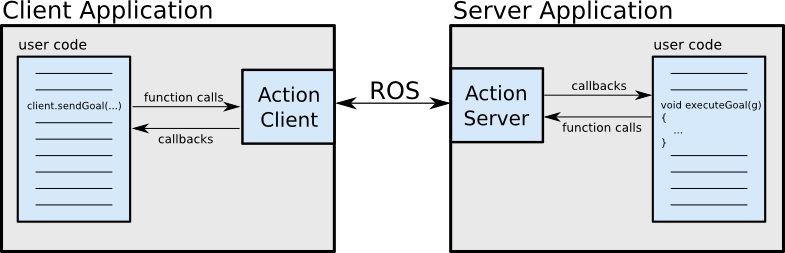
\includegraphics[width=0.8\textwidth]{client_server_interaction}
	\caption{Interaktion Client und Server}{Interaktion Client und Server\cite{actionli12:online}}
	\label{fig:clientServerInteraction}
\end{figure}

\subsection{Bags}
Bags werden in ROS gebraucht um die Daten, welche über eine Message verschickt werden zu speichern. Bags werden nicht aktiv für den Ablauf von Programmen benötigt, sind aber sehr hilfreich um Sensor- und Prozessdaten zu speichern und anschliessend auszuwerten.

\section{ROS Communityebene}
Für ROS ist, aufgrund des Open Source Aspekts, die Community ein sehr wichtiger Bestandteil des ganzen Projektes. Die ROS Community enthält ein extrem grosses Wissens- und Erfahrungspotential, dieses Wissen und die Erfahrungen wird von den einzelnen Gruppen der Community online zur Verfügung gestellt. Dazu stehen mehrere Möglichkeiten zur Verfügung:
\begin{itemize}
	\item Repositories
	\item ROS-Wiki unter \url{http://wiki.ros.org/}
	\item Bug Ticket System
	\item Mailverteiler
	\item Die 'ROS Answers'-Website	
\end{itemize} 
Das ROS-Wiki ist eine vom ROS-Konsortium erstellte Website, welche nahezu für alles ein vollständige Dokumentationen und Tutorials, mindestens aber Kurzbeschriebe, bereithält. Die ROS Answers Website bietet allen Anwendern von ROS eine Plattform in Form eines Forums um Fragen zu stellen und diese zu beantworten. Mithilfe dieser beiden Webseiten lassen sich fast alle Probleme und Unklarheiten, welche mit ROS in Verbindung stehen meistens klären.

\section{Standard Masseinheiten}
In ROS muss immer wieder mit Längen und Winkeln gearbeitet werden. Aus diesem Grund ist in ROS ein Standardisiertes Einheitensystem vorhanden. 
\begin{table}[h!]
\centering
\begin{tabular}{ll|ll}
\textbf{Grösse} & \textbf{Einheit} & \textbf{Grösse} & \textbf{Einheit} \\ \cline{1-3}
Länge           & Meter            & Leistung        & Watt             \\
Masse           & Kilogramm        & Spannung        & Volt             \\
Zeit            & Sekunden         & Temperatur      & Celsius          \\
Strom           & Ampere           & Magnetismus     & Tesla            \\
Winkel          & Radiant          & Frequenz        & Herz             \\
Kraft           & Newton           &                 &                 
\end{tabular}
\caption{Standard Masseinheiten in ROS}{Standard Masseinheiten in ROS\cite{REP103St88:online}}
\label{tab:StandardMasseinehiten}
\end{table}
\subsection{Quaternionen}
In ROS werden Rotationen nicht mit Eulerwinkeln gerechnet sondern in Quanternionen. Der grosse Vorteil von Quanternionen gegenüber der Verwendung von Eulerwinkeln ist, das bei den Quanternionen kein \gls{gimballock} entstehen kann. Quanternionen sind wie folgt definiert:
\begin{align*}
[w, x, y, z] =& [cos(\varTheta/2), sin(\varTheta/2) * nx, sin(\varTheta/2)* ny, sin(\varTheta/2) * nz]\\
\varTheta =& \text{Drehwinkel}\\
[nx,ny,nz] =& \text{Achse der Rotation}
\end{align*}

\section{Catkin}
Catkin ist das Standard Build-Tool von ROS. Catkin kombiniert CMakemakros und Pythonskripts um dem normalen CMake einige neue Funktionalitäten hinzuzufügen. Catkin wurde erstellt um das vorherige Build-Tool rosbuild abzulösen, catkin ermöglicht es Pakete mithilfe von 'find package' zu finden und mehrere voneinander abhängige Projekte gleichzeitig zu compilieren.\\
ROS nutzt ein eigenes Build-Tool um es zu ermöglichen, dass alle Pakete in ROS, unabhängig von ihrer Programmiersprache, ohne Probleme compiliert werden können. Es wird mit catkin ermöglicht voneinander abhängige Pakete zu compilieren, welche mit unterschiedlichen Programmiersprachen geschrieben wurden, andere Tools benötigen und/oder andern Organisationsstrukturen unterliegen. \cite{Allen2016}
\subsection{Workspace}
Catkin benötigt einen eigenen Workspace, welcher wie folgt initialisiert werden kann: \\
(Hier als Beispiel im Homedirectory im Ordner catkin\_ws)

\begin{code}
	\begin{minted}{bash}
	$ source /opt/ros/kinetic/setup.bash
	$ mkdir -p ~/catkin_ws/src
	$ cd ~/catkin_ws/
	$ catkin_make
	\end{minted}
	\vspace{-15pt}
	\caption{Setup eines catkin Workspace}
	\label{code:CatkinWS}
\end{code}
Anschliessend ist es zu empfehlen, dass die Variable 'ROS\_PACKAGE\_PATH' so gesetzt wird, dass der Workspace erkannt wird:

\begin{code}
	\begin{minted}{bash}
	$ echo $ROS_PACKAGE_PATH
	/home/youruser/catkin_ws/src:/opt/ros/kinetic/share
	\end{minted}
	\vspace{-15pt}
	\caption{Setzen der Umgebungsvariable}
	\label{code:PathVariable}
\end{code}

\subsection{CMakeLists}\label{Anhang:catkinCMakeLists}
Jedes Package in ROS benötigt zum compilieren durch catkin eine CMakeLists.txt Datei in ihrem Ordner. In dieser Datei werden diverse zum compilieren benötigte Einstellungen vorgenommen, unter anderem wird angegeben wo die Standard ROS-Packages zu finden sind, welche Packages zum compilieren Notwendig sind, welche der Files einen Node bilden und auch Abhängigkeiten können definiert werden. Zudem wird dem Compiler hier mitgeteilt, aus welchen Files Messages oder Services generiert werden sollen. Es ist zudem möglich und sehr zu empfehlen Flags zu setzen, welche erweiterte Fehlermeldungen bei Kompilierfehlern ausgeben. Dies vereinfacht ein Debuggen Nachfolgend sind einige der wichtigsten Zeilen aus einem CMakeFile.txt aufgeführt. Ein vollständiges CMakeFile kann im Anhang unter \ref{Anhang:Cmakelists} gefunden werden. \cite{Allen2016} \\

\begin{minipage}[H]{\textwidth}
	\begingroup
	\parfillskip=0pt
	% zwei weitere Minipages
	\begin{minipage}[t]{0.47\textwidth}        
\begin{code}
	\begin{minted}{cmake}
	find_package(catkin REQUIRED COMPONENTS
		roscpp
		geometry_msgs
		moveit_core
		moveit_ros_planning
		moveit_ros_planning_interface
		pluginlib
		cmake_modules
		message_generation
		genmsg
	)	
	\end{minted}
	\vspace{-15pt}
	\caption{Für das compilieren benötigte ROS-Packages}
	\label{code:ROSPackages}
\end{code}
	\end{minipage}%
	\hfill
	\begin{minipage}[t]{0.47\textwidth}
		\begin{code}
			\begin{minted}{cmake}
			add_executable(NodeName
				src/myROSNode.cpp
			)			
			\end{minted}
			\vspace{-15pt}
			\caption{Definieren eines Nodes aus einem .cpp-File}
			\label{code:CatkinCpp}
			
		\begin{code}
			\begin{minted}{cmake}
			add_library(LibraryName
				src/myLibrary.cpp
			)			
			target_link_libraries(targetName
				${catkin_LIBRARIES}
				LibraryName
			)			
			\end{minted}
			\vspace{-15pt}
			\caption{Hinzufügen und verlinken von Bibliotheken}
			\label{code:catkinBib}
		\end{code}
		\end{code}  
	\end{minipage}%
	\par\endgroup
\end{minipage}

\subsection{Package File} \label{sec:catkinPackageFile}
Das Package File package.xml wird von catkin gebraucht um Metadaten zu definieren. Diese beinhalten Versionsnummer, Paketname, Ersteller/Unterhalter und Lizenzen. Zudem muss angegeben werden welche anderen Packages vor dem compilieren bereits compiliert sein müssen (build\_depend), welche Packages zum compilieren benötigt werden (buildtool\_depend) und welche Packages während der Laufzeit (run\_depend) des Packages benötigt werden. Folgend ein Minimalbeispiel einer package.xml Datei. \cite{Allen2016}
\begin{code}
	\begin{minted}{xml}
<?xml version="1.0"?><package>
	<name>myPackage</name>
	<version>0.0.1</version>
	<description>My personal ROS-Package. Which does...</description>

	<maintainer email="Hans.Muster@example.com">Hans Muster</maintainer>

	<license>BSD</license>
	
	<author email="Hans.Muster@example.com">Jane Doe</author>

	<buildtool_depend>catkin</buildtool_depend>
	<build_depend>roscpp</build_depend>
	<run_depend>roscpp</run_depend>
	<build_depend>moveit_core</build_depend>
	<run_depend>moveit_core</run_depend>
	<build_depend>moveit_ros_planning_interface</build_depend>
	<run_depend>moveit_ros_planning_interface</run_depend>

	<!-- The export tag contains other, unspecified, tags -->
	<export>
	<!-- Other tools can request additional information be placed here -->
	</export>
</package>
	\end{minted}
	\vspace{-15pt}
	\caption{Minimalbeispiel einer package.xml Datei}
	\label{code:PackageXML}
\end{code}

\section{URDF}\label{sec:URDF}
Das \gls{URDF} wird gebraucht um die physikalischen Eigenschaften eines Roboters zu beschreiben. Ein URDF besteht aus einer Zusammenstellung von Links (Gliedern) und Joints (Gelenken) um eine Kinematische Kette zu bilden. (siehe Abb. \ref{fig:URDFKin})
\begin{figure} [h]
	\begin{minipage}[h]{0,49\textwidth}
		\centering
		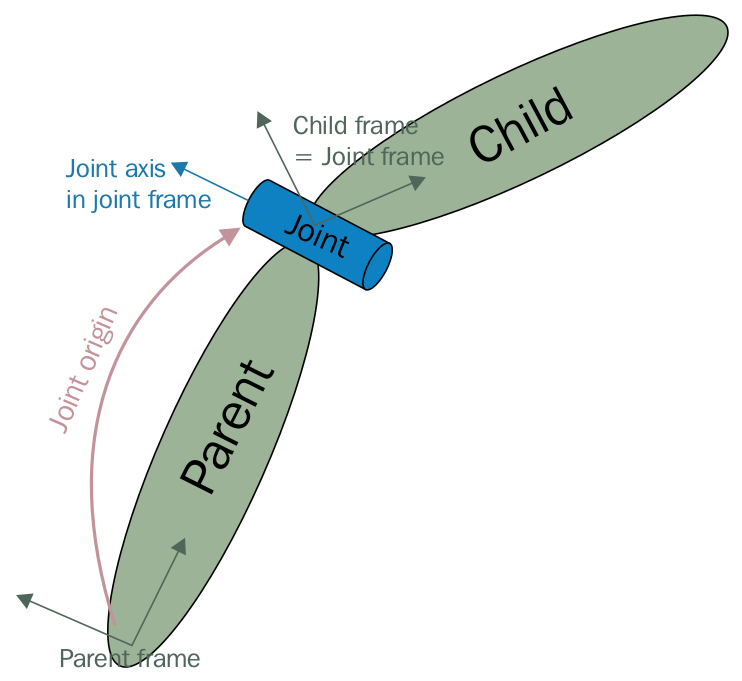
\includegraphics[width=0.95\textwidth]{URDF_kin}
		\caption[Symbolische Darstellung einer Kinematischen Kette]{Symbolische Darstellung einer Kinematischen Kette \cite{Joseph2015}}
		\label{fig:URDFKin}
	\end{minipage}
	\begin{minipage}[h]{0,49\textwidth}
		\centering
		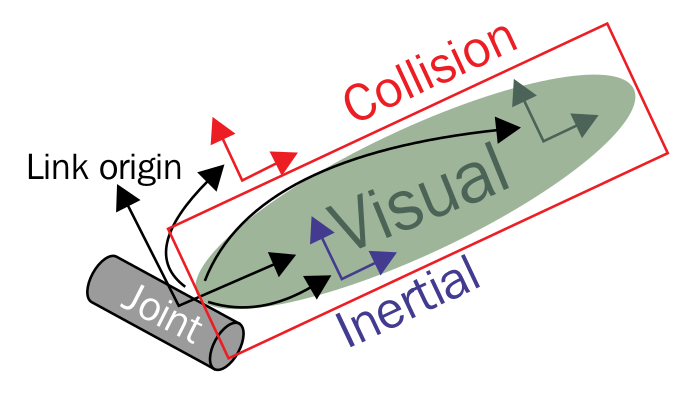
\includegraphics[width=0.95\textwidth]{URDF_link}
		\caption[Symbolische Darstellung eines Links]{Symbolische Darstellung eines Links \cite{Joseph2015}}
		\label{fig:URDFLink}
	\end{minipage}
\end{figure}

\subsection{Links}
Für jeden Link muss dabei ein Koordinatensystem und ein Geometrisches Modell definiert sein. Optional ist es möglich Massenträgheitsmomente, Farben und eine simplere Geometrie für die Kollisionsüberwachung zu definieren. Für die Geometrien ist es zudem möglich, die 3D-Objekte über importierte .stl-Files zu generieren.
\begin{code}
	\begin{minted}{xml}
<link name="base_link">
	<inertial>
		<mass value="6.215"/>
		<origin rpy="0 0 0" xyz="-0.04204 8.01E-05 0.07964"/>
		<inertia ixx="0.0247272" ixy="-8.0784E-05" ixz="0.00130902" iyy="0.0491285" iyz="-8.0419E-06" izz="0.0472376"/>
	</inertial>
	<visual>
		<origin rpy="0 0 0" xyz="0 0 0"/>
		<geometry>
			<mesh filename="package://abb_irb120_support/meshes/irb120_3_58/visual/base_link.stl"/>
		</geometry>
		<material name="">
			<color rgba="0.7372549 0.3490196 0.1607843 1"/>
		</material>
	</visual>
	<collision>
		<origin rpy="0 0 0" xyz="0 0 0"/>
		<geometry>
			<mesh filename="package://abb_irb120_support/meshes/irb120_3_58/collision/base_link.stl"/>
		</geometry>
		<material name="">
			<color rgba="1 1 0 1"/>
		</material>
	</collision>
</link>	
	\end{minted}
	\vspace{-15pt}
	\caption{Beispiel eines voll definierten Links anhand der Basis des ABB IRB120}
	\label{code:URDFLink}
\end{code}

\subsection{Joints}
Für einen Gelenk (Joint) muss definiert werden um welche Achsen sich das Gelenk drehen darf und welche beiden Links das Gelenk verbindet. Optional können Endanschläge, maximale Geschwindigkeiten, Reibungs- und Dämpfungskonstanten definiert werden. Mögliche Definitionen von Drehachsen sind revolute, continuous, prismatic, fixed, floating und planar. Nachfolgend ist ein Codeausschnitt aufgeführt, welcher ein vollständig definiertes Gelenk beschreibt.
\begin{code}
	\begin{minted}{xml}
<joint name="joint_1" type="revolute">
	<origin rpy="0 0 0" xyz="0 0 0"/>
	<parent link="base_link"/>
	<child link="link_1"/>
	<limit effort="0" lower="-2.87979" upper="2.87979" velocity="4.36332"/>
	<axis xyz="0 0 1"/>
	<dynamics damping="0.0" friction="0.0"/>
</joint>
	\end{minted}
	\vspace{-15pt}
	\caption{Beispiel eines Rotationgelenkes}
	\label{code:URDFJoint}
\end{code}

\section{MoveIt!}
MoveIt!ist eine Software zur Bewegungsplanung, Manipulation, 3D Wahrnehmung, Kinematik, Steuerung und Navigation. Es basiert auf einer Pluginstruktur, welche von ROS übernommen wurde. Dies ermöglicht es, dass MoveIt! sehr Ressourcenschonend ist und jeweils nur die Teile aktiv sind, welche auch für die jeweilige Anwendung nötig sind. Zudem ist es möglich die move\_group einfach über neue Plugins zu erweitern. Der zentrale Node in MoveIt! ist der move\_group Node, auf die Services und Actions dieses Nodes können über drei mögliche Arten zugegriffen werden:\cite{Chitta2016}

\begin{figure}[h!]
	\centering
	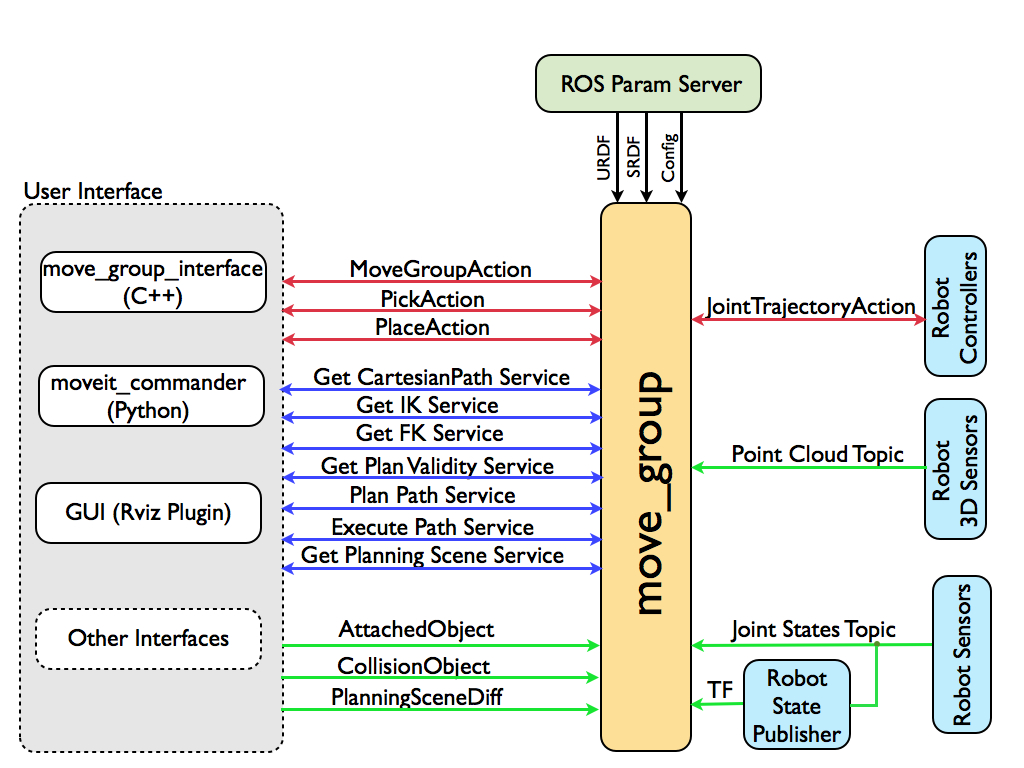
\includegraphics[width=0.8\textwidth]{move_group}
	\caption[move\_group Architektur]{move\_group Architektur\cite{Concepts23:online}}
	\label{fig:move_group}
\end{figure}

\paragraph{move\_group\_interface}
Das move\_group\_interface bietet eine API für \verb|C++|, diese eignet sich vor allem für die Erstellung komplexer Anwendungen. 
\paragraph{moveit\_commander}
Das moveit\_commander Package bietet eine API für \verb|Python|, welche sich vor allem für das erstellen von einfachen Skripts eignet. 
\paragraph{RVIZ}
Mithilfe eines Plugins für RVIZ, dem ROS eigenen Visualisierungspackage, kann die move\_group direkt über ein \gls{GUI} gesteuert werden. Dies eignet sich vor allem für schnelles Visualisieren oder das Aufsetzen eines Roboters. 

\subsection{Konfiguration}
Beim Start einer neuen move\_group bezieht diese direkt beim Parameterserver von ROS benötigte Dateien. Diese beinhalten eine URDF Datei(siehe Abschnitt \ref{sec:URDF}, welche die Physikalische Beschreibung des zu steuernden Roboters enthält. Ergänzend zum URDF wird ein SRDF benötigt, welches zusätzliche Informationen über den Roboter enthält, welche beim erstellen eines MoveIt!-Packages (siehe Abschnitt \ref{sec:ImplementierungMontage}) definiert werden. Die beiden Files (URDF und SRDF) müssen zwingend auf dem Parameterserver von ROS abgelegt sein. Zusätzlich sucht die move\_group auf dem Parameterserver noch nach weiteren, nicht zwangsweise vorhandenen, Konfigurationen. Diese können unter anderem maximale Gelenkgeschwindigkeiten, -beschleunigungen und -winkel enthalten sowie auch Daten über die Umgebung. \cite{Concepts23:online}

\subsection{Roboterinterface}
Über das Roboterinterface kommuniziert die move\_group mithilfe von ROS Topics und Actions mit dem ausgewählten Roboter.

\subsubsection{Joint State  und Transformations Informationen}
Zur Bestimmung der momentanen Position des Roboters hört die move\_group auf dem Topic /joint\_states, nach publizierten Gelenkpositionen. Diese Information geht auch über den Node Robot State Publisher welcher mithilfe eines Kinematischen Models die einzelnen Gelenkwinkel in eine genaue Position der jeweiligen Koordinatensysteme des Roboters umrechnet. Somit stehen der move\_group jederzeit die einzelnen Gelenkwinkel sowie auch die Position jeder Achse des Roboters zur Verfügung.\cite{Joseph2015}

\subsubsection{Controller Interface}
Die move\_group sendet Bewegungsbefehle über das FollowJointTrajectoryAction Interface, welches von ROS zur Verfügung gestellt wird, auf den entsprechenden Roboter Controller. Dabei ist zu beachten, dass auf dem Controller vorgängig ein entsprechender Actionserver implementiert werden muss, welcher die Anfragen in Steuerungsbefehle umwandelt. \cite{Joseph2015}

\subsection{MoveIt! Setup Assistant}
Der MoveIt! Setup Assistant ist ein sehr hilfreiches Tool welches ermöglicht jegliche Art von Roboter zu Konfigurieren so, dass dieser anschliessend mit MoveIt! respektive der move\_group gebraucht werden kann. Dazu benötigt der Setup Assistant ein gültiges URDF-File, aus welchem ein SRDF-File und andere für MoveIt! und die Bewegungsplanung benötigten Files generiert werden. Dank dem \gls{GUI} des Setup Assistants wird einem das erstellen des configuration packages sehr erleichtert. Dazu müssen folgende Schritte abgearbeitet werden:\cite{Industri70:online}
\begin{enumerate}
	\itemsep0pt
	\item Starten und URDF laden
	\item Generieren der Selbstkollisionsmatrix
	\item Virtuelle Gelenke hinzufügen
	\item Planungsgruppen erstellen
	\item Roboterposen hinzufügen
	\item Endeffektoren hinzufügen
	\item Passive Gelenke hinzufügen
	\item Konfigurationsfiles generieren	
\end{enumerate}
Der Setup Assistant kann über ein Linux Terminal mit folgendem Befehl gestartet werden:\\
\mintinline{bash}{$ roslaunch moveit_setup_assistant setup_assistant.launch}\\ %$
Eine ausführlichere Beschreibung anhand eines Beispiels ist im Abschnitt \ref{sec:MoveitSetup} aufgeführt.

\subsection{Planningscene}
Die Planningscene beinhaltet eine Repräsentation der echten Welt, in ihr ist der Roboter in seinem momentanen Zustand abgebildet, sowie auch alle Objekte welche sich momentan im Arbeitsraum des Roboters befinden. Die Planningscene wird für die Bestimmung von Kollisionsberechnungen gebraucht. \cite{Pan2012}

\subsection{Kollisionsüberwachung}
Auch für die Kollisionsüberwachung wird eine Bibliothek über ein Plugin implementiert, standardmässig ist dies die \gls{FCL}. Dabei werden die folgenden Geometrischen Formate unterstützt:\cite{Pan2012}
\begin{itemize}
	\itemsep0pt
	\item Meshes: .stl oder .dae
	\item Primitive Shapes: Boxen, Zylinder, Kugeln, etc.
	\item \gls{octomap}: kann direkt für Kollisionsüberwachung gebraucht werden
\end{itemize}
Beim erstellen eines neuen MoveIt! Packages kann mithilfe des MoveIt! Setup Assistants eine Kollisionsmatrix erstellt werden, welche definiert welche Körper für die Berechnung der Kollision vernachlässigt werden können weil sie zum Beispiel gar nicht kollidieren können. Dies erspart einen grossen Teil an Rechenleistung und somit können Bahnplanungen schneller durchgeführt werden.\cite{Chitta2016}

\subsection{Kinematischer Solver}
Zur Lösung von Kinematikberechnungen sind in MoveIt! standardmässig zwei numerische kinematische Solver über ein Plugin implementiert.\cite{Chitta2016} Bei diesen Solvern handelt es sich um KDL und LMA beide basieren auf der \gls{KDL} von Orocos.\cite{Kinemati93:online} Zusätzlich wurde der Planer Trac-IK von Traclabs installiert, welcher laut den Angaben von Traclabs massiv schneller und zuverlässiger Lösungen finden soll, als die beiden Standardsolver.\cite{traclabs28:online} Es muss je nach Roboter ausgetestet werden, welcher Solver bessere Ergebnisse liefert.

\subsection{Bewegungsplanung}
MoveIt! implementiert Bewegungsplaner über ein Plugin, dies ermöglicht es einfach zwischen mehreren Bewegungsplanungsbibliotheken zu wechseln, gleichzeitig ist es möglich einen eigenen Anwendungsspezifischen Bewegungsplaner in MoveIt! zu implementieren. Die Standard mässig implementierte Planungsbibliothek ist \gls{OMPL}. Mithilfe des MoveIt! Setup Assistant können die einzelnen Planer Konfiguriert werden.\cite{Chitta2016} \\

Um ein Grundverständnis für die Planer zu entwickeln wird in diesem Abschnitt kurz auf die in OMPL verfügbaren Planer eingegangen, aufgrund der Komplexität der Planer wird auf eine ausführlichere Beschreibung verzichtet. 
Grundsätzlich können die Planer welche in \gls{OMPL} vorhanden sind in zwei Kategorien unterteilt werden. Es gibt geometrische Planer und Kontrollbasierte Planer.\cite{Availabl94:online}
\subsubsection{Geometrische Planer}
Geometrische Planer berücksichtigen bei der Bahnplanung nur geometrische und kinematische Beschränkungen. Dabei trifft der Planer die Annahme, dass jeder vom Bahnplaner gefundene Weg in eine Bahn umgewandelt werden kann welche Dynamisch auch fahrbar ist. Dabei können diese Planer wieder  in folgende Unterkategorien unterteilt werden:\cite{Availabl94:online}
\paragraph{Single-query Planer} Diese Planer bauen eine Baumstruktur auf, welche aus gültigen Bewegungen besteht und sich vom Start in Richtung Ziel bewegen. Einige Planer bauen die Baumstruktur gleichzeitig von Ziel und Start auf und treffen sich in der Mitte. Die einzelnen Planer dieses Typs unterscheiden sich hauptsächlich darin, wann und wo die Baumstruktur erweitert wird.\cite{Availabl94:online}
\paragraph{Multi-query Planer} Diese Art von Planern erstellt vorgängig eine Karte der ganzen Umgebung, welche anschliessend genutzt wird um zu bestimmen ob sich die berechneten Bewegungen innerhalb dieser Karte befinden und somit gültig sind.\cite{Availabl94:online}
\paragraph{Optimierende Planer} Optimierende Planer wählen gefundene Wege aufgrund von Optimierungskriterien, normalerweise ist dies die Distanz welche kurz gehalten werden soll. Es ist jedoch auch möglich, zum Beispiel die mechanische Arbeit zu minimieren. Obwohl das finden eines optimalen Weges von Vorteil ist, ist zu beachten, dass optimierende Planer die ihnen zur Verfügung gestellte Rechenzeit in der Regel komplett ausnutzen. Somit sind die gefahrenen Wege meistens kürzer als bei den Queryplanern es ist aber möglich, dass die gesparte Fahrzeit in längerer Rechenzeit verloren geht.\cite{Lav06}

\subsubsection{Kontrollbasierte Planer}
Kontrollbasierte Planer setzen nicht nur auf geometrische und kinematische Beschränkungen. Es werden Zustandsdarstellungen benutzt, um einzelne Positionen auf dem Weg zu definieren. Über Algorithmen wird bewertet wie hoch der Steuerungsaufwand ist um von Zustand zu Zustand zu gelangen, dieser soll möglichst klein gehalten werden. \cite{Availabl94:online}

\subsection{Trajektorienberechnung}
Die aus der Bewegungsplanung berechneten Bahnen beinhalten noch keine Zeitinformationen, aus diesem Grund ist in MoveIt! ein Plugin zur Trajektorienberechnung implementiert. Dieses Plugin berechnet aufgrund der in den Konfigurationsdateien abgespeicherten erlaubten Gelenkgeschwindigkeiten aus der berechneten Bahn eine Trajektorie. Auch hier ist es wieder möglich, über ein Plugin eine eigene Version der Trajektorienberechnung zu implementieren. \cite{Chitta2016}

\section{ROS Industrial}
ROS-Industrial erweitert das von ROS zur Verfügung gestellte Framework rund um Industrierobotik und -automation. Die Erweiterung durch ROS-Industrial umfasst eine Vielzahl von Interfaces für diverse in der Industrie gebräuchliche Hardware, wie zum Beispiel Greifer oder Sensoren. Zudem sind in dem ROS-Industrial Repository\footnote{https://github.com/ros-industrial/} diverse Bibliotheken verfügbar, welche die spezifisch auf die Anwendung im Rahmen der Industrie zugeschnitten sind. ROS-I wird durch ein Konsortium\cite{ROS-IMembers} an Forschergruppen sowie auch von Firmen aus der Industrie unterstützt.
Folgend sind einige Vorteile und Eigenschaften, der ROS-I Beschreibung aufgeführt:\cite{Descript37:online}
\begin{itemize}
	\itemsep0pt
	\item Implementiert die bereits mächtigen Funktionen aus ROS
	\item Ermöglicht neue Applikationen
	\item Vereinfacht die Roboterprogrammierung bis auf die Taskebene
	\item Reduziert Kosten
	\item Open Source
\end{itemize}
ROS-Industrial kann grundsätzlich in zwei Pakettypen unterteilt werden. Zum einen gibt es die ROS-I spezifischen Pakete, diese beinhalten alle generell in ROS-I brauchbaren Funktionen. Zum anderen gibt es die herstellerspezifischen Pakete, diese beinhalten die benötigten Beschreibungs- sowie Setupfiles, um einen Roboter eines bestimmten Herstellers in Betrieb zu nehmen. 
\subsection{Unterstützte Hersteller}
ROS-I arbeitet eng mit diversen Forschungseinrichtungen sowie auch Herstellern zusammen und unterstützt bereits von Haus aus diverse Hardware von einigen Herstellern. Gleichzeitig gibt es eine sehr grosse Anzahl an Paketen und Bibliotheken, welche durch die Open Source Community erstellt wurden aber nicht offiziell - oder zumindest noch nicht - von ROS-I unterstützt werden.
\begin{table}[H]
	\centering
	\begin{tabular}{llll}
		\textbf{Hersteller} & \textbf{Controller(s)} & \textbf{Manipulator} & \textbf{MoveItPkg} \\ \hline
		ABB                 & IRC5                   & IRB-2400             & YES                \\
		                    &                        & IRB-5400             & NO                 \\ \hline
		Adept               & CX, CS                 & Viper 650            & NO                 \\ \hline
		Fanuc               & R-30iA / R-30iB        & LR Mate 200iC (all)  & YES                \\
		                    &                        & LR Mate 200iD        & YES                \\
		                    &                        & M-10iA               & YES                \\
		                    &                        & M-16iB/20            & YES                \\
		                    &                        & M-20iA(/10L)         & YES                \\
		                    &                        & M-430iA/(2F, 2P)     & YES                \\
		                    &                        & M-900iA/260L 5       & NO                 \\ \hline
		Motoman             & DX100                  & SIA10D/F             & NO                 \\
		                    &                        & FS100                & NO                 \\
		                    &                        & DX200                & NO                 \\
		                    &                        & YRC1000              & NO                 \\ \hline
		Universal Robot     & CB2/CB3 10             & UR 5                 & YES                \\
		                    &                        & UR 10                & YES                \\ \hline
	\end{tabular}
	\caption[Offiziell unterstützte Hardware]{Offiziell unterstützte Hardware\cite{HardwareSup:online}}
	\label{tab:hersteller}
\end{table}

\subsection{Robot Support Package}
Robotsupportpackages werden von ROS-Industrial verwendet um alle Dateien an einem Ort zu sammeln, welche nötig sind um einen Industrieroboter zu betreiben, respektive eine MoveIt! Konfiguration dafür zu erstellen. Die Strukturen, Namensgebungen sowie auch Funktionen in einem ROS-I Package unterliegen in diverser Konvention. 
\subsubsection{Ordnerstruktur}
Übersichtshalber ist der Inhalt solcher Packages definiert, es wird auch empfohlen beim erstellen solcher Packages sich an die Ordnerstruktur sowie an die Namenskonventionen zu halten. Die Ordnerstruktur sieht in folgendermassen aus:\\
\dirtree{%
	.1 RoboterName\_support.
	.2 config.
	.2 launch.
	.2 meshes.
	.2 test.
	.2 urdf.
}
\subsubsection{Launchfiles}
Durch ROS-Industrial werden einige .launch-Files vorgegeben, welche in jedem Support Package vorhanden sein müssen. Diese werden teils automatisch generiert, andere müssen selber geschrieben werden. Nachfolgend eine Auflistung der .launch-Files und eine kurze Beschreibung ihrer Funktion.
\begin{description}
	\item[load\_roboterName.launch] Lädt alle roboterspezifischen Konfigurationsdateien, welche von MoveIt! benötigt werden auf den ROS Parameterserver.
	\item[test\_roboterName.launch] Startet RVIZ und ermöglicht es die Konfiguration der Gelenke zu überprüfen. Dafür werden die beiden Nodes joint\_state\_publisher und robot\_state\_publisher gestartet.
	\item[robot\_state\_visualize\_roboterName.launch] Visualisiert den Zustand eines echten oder simulierten Roboters in RVIZ. Es können dem Robotercontroller dabei keine Befehle erteilt werden.
\end{description}
Das letzte .launch-File ist das robot\_interface welches eine bidirektionale Kommunikation mit dem Robotercontroller startet. Dieses .launch-File gibt es in zwei unterschiedliche Versionen, abhängig vom Controller. Diese unterscheiden sich darin, wie ROS-I mit dem Robotercontroller kommuniziert. 
\begin{description}
	\item[robot\_interface\_download\_roboterName.launch] Das Download Interface sendet die gesamte berechnete Trajektorie in einem Paket an den Controller, dieser führt diese Anschliessend aus. Beim Erhalt eines neuen Trajektorienpakets wird der Roboter gestoppt und die alte Trajektorie verworfen. 
	\item[robot\_interface\_streaming\_roboterName.launch] Beim Streaming Interface werden die generierten Trajektorienpunkte direkt an den Controller gesendet, welcher leicht Zeitverzögert die ankommenden Trajektorienpunkte ausführt.
\end{description}

\subsection{Standardisierte Links}
Gemäss ROS-I sind drei Links definiert, welche in jedem Package gleich benennt sein müssen. Einerseits der base\_link welcher die Basis des Roboters bildet, an welcher dieser befestigt wird. Der tool0 Link ist der letzte Link eines Roboters, er befindet sich somit im Zentrum des \gls{TCP}, seine Orientierung entspricht der Orientierung des Standard Toolframes des Roboters. Der dritte definierte Link ist der flange\_frame, gemäss der Definition von ROS-I entspricht seine Position dem Befestigungspunkt des jeweiligen Endeffektors. Die Orientierung ist genormt mit der x-Achse in Vorwärtsrichtung, y nach links und z nach oben.

\subsection{URDF's und xacro}
Die physikalischen Beschreibungen eines industriellen Roboters werden nicht in einem URDF verfasst, sondern in einem .xacro-File. Diese sind vom Syntax her identisch, jedoch erlauben es .xacro-Files Macros zu verwenden. Mithilfe von Macros können Tags generiert werden, welche es ermöglichen andere .xacro-Files zu suchen und Importieren. Zudem ist es möglich jedem Gelenk und Glied eines Roboters ein Präfix zu geben. Dies verhindert bei mehrfacher Verwendung eines .xacro-Files Namenskonflikte, falls ein xacro mehrfach verwendet werden will.
Aus einem .xacro-File muss kann anschliessend wieder ein URDF generiert werden. 